{
\usebackgroundtemplate{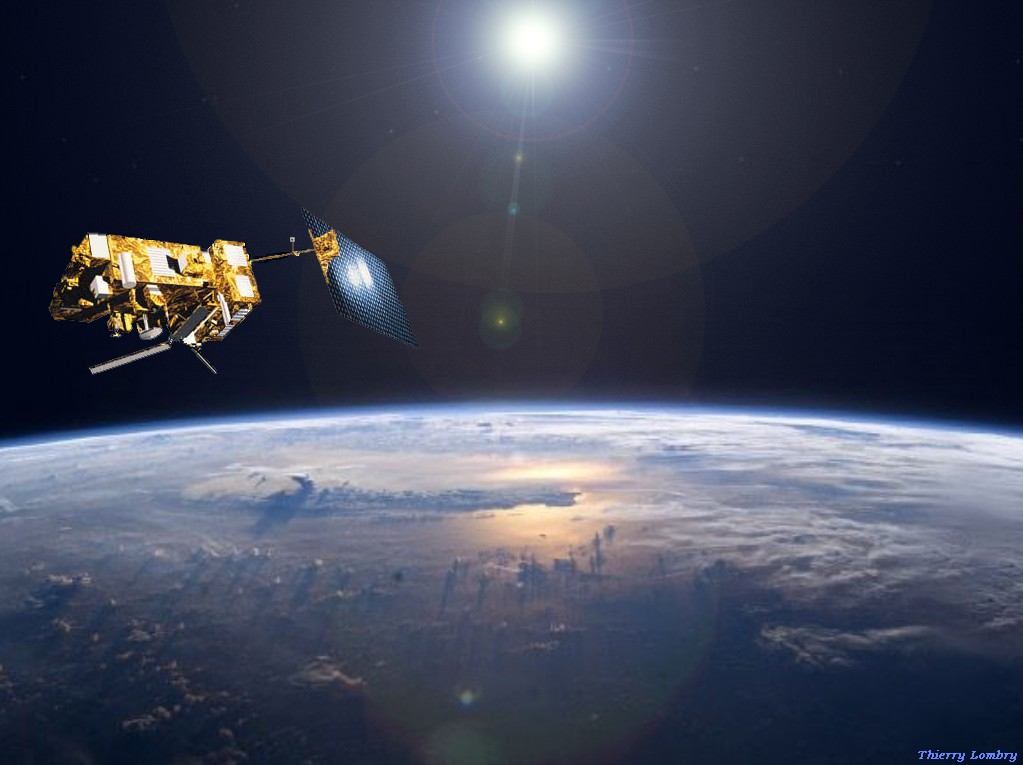
\includegraphics[height=\paperheight, keepaspectratio]{images/low_orbit}}%
\begin{frame}
\end{frame}
\begin{frame}
    \frametitle{About that circulizing}
    \begin{block}{}
        We are now almost in low earth orbit but still falling down. Our periapsis may still be within the atmosphere.
        So we need to learn how to manipulate our orbit while in space.
    \end{block}
    \begin{block}{Basics}
        Movement on an orbit generally affects the oposite side of the orbit.
    \end{block}
\end{frame}
\begin{frame}
    \frametitle{Adjusting Orbits}
    \begin{block}{}
        \begin{center}
            At any point on the orbit you can burn in 3 directions. up/down, left/right, forwards/backwards
        \end{center}
    \end{block}
    \begin{block}{}
        \begin{center}
            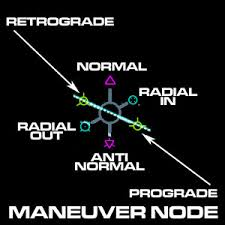
\includegraphics[scale=0.8]{images/maneuver_node}
        \end{center}
    \end{block}
\end{frame}
\begin{frame}
    \frametitle{Low Orbit}
    \begin{block}{Maveuvering in space}
        \begin{description}
            \item [prograde] Along your movement vector, used to increase orbit altitude
            \item [retrograde] Oposite your movement vector, used to decrease orbit altitude
            \item [normal] Perpendicular to orbit, used to increase/decrease inclination
            \item [anti-normal] perpendiculat to orbit, used to increase/decrease inclination
            \item [radial] Towards parent body, Used to shift orbit around
            \item [anti-radial] Away from parent body, used to shift orbit around
        \end{description}
    \end{block}
\end{frame}
}

\begin{frame}
    \frametitle{Prograde}
    \begin{center}
        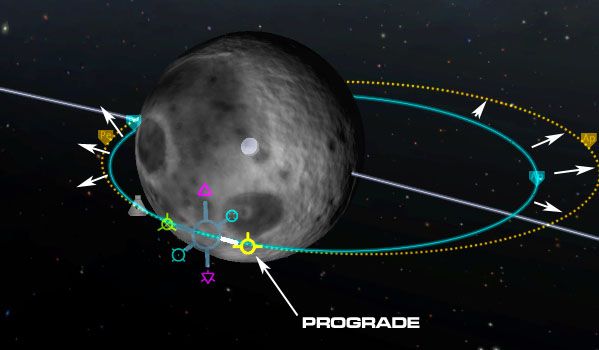
\includegraphics[scale=0.5]{images/prograde}
    \end{center}
\end{frame}
\begin{frame}
    \frametitle{Normal}
    \begin{center}
        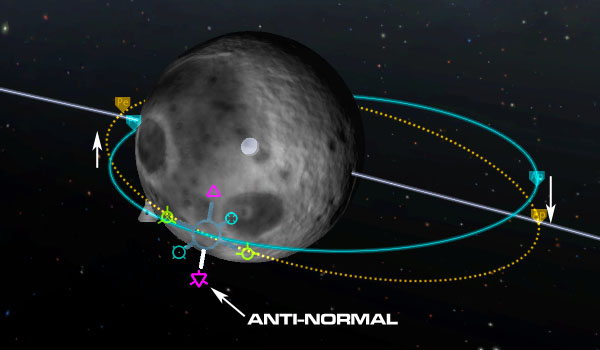
\includegraphics[scale=0.5]{images/anti_normal}
    \end{center}
\end{frame}
\begin{frame}
    \frametitle{Radial}
    \begin{center}
        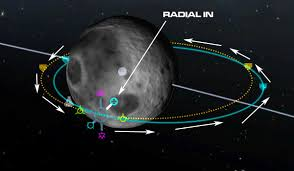
\includegraphics[]{images/radial}
    \end{center}
\end{frame}
